% $Id: calibration.tex 9912 2022-03-20 19:17:14Z mskala $

%
% Firmware update and calibration
% Copyright (C) 2022  Matthew Skala
%
% This program is free software: you can redistribute it and/or modify
% it under the terms of the GNU General Public License as published by
% the Free Software Foundation, version 3.
%
% This program is distributed in the hope that it will be useful,
% but WITHOUT ANY WARRANTY; without even the implied warranty of
% MERCHANTABILITY or FITNESS FOR A PARTICULAR PURPOSE.  See the
% GNU General Public License for more details.
%
% You should have received a copy of the GNU General Public License
% along with this program.  If not, see <http://www.gnu.org/licenses/>.
%
% Matthew Skala
% https://northcoastsynthesis.com/
% mskala@northcoastsynthesis.com
%

\chapter{Firmware update and calibration}

Many of the Gracious Host's features are defined by \emph{firmware} -- that
is software built into the hardware -- and it is possible to replace the
firmware on an existing module with a new version.  Before attempting a
firmware update you should make sure you know \emph{why} you are updating
your firmware.  If your module works and you are satisfied with it, you may
not need to make any changes.  The update process involves some risk and
should not be attempted for no reason.  But it is possible that I, or third
parties, may release enhanced firmware with special features in the future. 
You may also have created new firmware of your own using the information in
the \emph{MSK~014 Gracious Host Programmer's Manual}.

After loading the firmware, the module also needs \emph{calibration}, which
adjusts the mapping between analog values in the outside world and digital
values used in the firmware, to account for component values and
module-to-module variation.  The calibration process is mostly automated.  It
involves using a standard V/oct VCO as a reference.

If you have built your own module, it will need to be calibrated.  Running
the firmware update is one way to accomplish that, but you can also plug in
a typing keyboard and enter maintenance code 5833, as described in the
chapter on typing keyboards, to run the calibration procedure without
updating firmware first.

To complete the update and calibration process, you will need:
\begin{itemize}
  \item The Gracious Host module;
  \item a V/octave VCO that can track reasonably well over 0V--5V control
    voltage input;
  \item a couple of patch cables and the necessary power supply to run both
    modules at once;
  \item a USB flash drive and computer capable of writing files to it; and
  \item the firmware image file you want to use.
\end{itemize}

\section{Preparing a firmware image}

You will need an \emph{image file}, which contains the executable firmware
code in a special format specific to the Gracious Host.  Up-to-date official
firmware images are available from the North Coast Synthesis Web site at
\url{https://northcoastsynthesis.com/}, as is the source code.  Third-party
firmware images may be available elsewhere.

The official firmware is subject to the GNU General Public License, and so
must be any others that include parts of it.  Among other things, that means
third-party distributors of installable binary images are required to
share their source code if their images contain any part of the original
firmware.

The process of loading new firmware depends on code included in the
\emph{old} firmware.  It is possible that loading a bad firmware image may
``brick'' your module, making it unable to load any further updates through
USB.  For that reason, you should be careful about loading unknown or
untested firmware images.  The module will not load an image file that fails
a check of the CRC32 values included in the file, so mere file corruption is
unlikely to result in a bricked module.  But buggy code correctly packaged
could possibly be a problem.

Prepare a USB flash drive in the format typically used by Windows.
Most other popular operating systems can also format flash drives
this way.  The default settings should work.  In more detail: the drive
needs to have at most $2^{32}$ blocks, which translates to a maximum
capacity of 2T if the blocks are standard 512-byte size; FAT12, FAT16, and
FAT32 should all work, with FAT32 having received the most thorough testing;
and the filesystem needs to be either written to the entire drive, or in a
primary (not extended) partition described by a standard DOS partition
table.

Rename the firmware to ``FIRMWARE.FRM'' if that is not already its name, and
put the file in the root directory of the flash drive.  The module will
ignore all subdirectories and all files with other names.

\section{Firmware update}

Power up the module, and insert the flash drive.  The module will
automatically detect the drive, scan it for a valid firmware file, and
attempt to reflash itself with the new image.  That normally takes less than
a second.  If the update succeeds, the module will start the calibration
process, below, with slow-flashing red LEDs.

If firmware update fails, the module will perform the \emph{failure
display}, which consists of both LEDs flashing red slowly (1\,Hz, 50\%\ duty
cycle) and an ominous tune played in 0V--9V square waves on the digital output
jacks.  If you patch either output jack to a speaker or headphone (beware of
the DC offset; putting it through an AC-coupled module of some kind might
help) you can hear this.

\qquad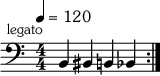
\includegraphics{failure.cropped.eps}

\blinkcodeLR{}{4/8}{}{4/8}

The failure display lasts one minute, after which (if you haven't powered it
off already) the module will reboot.  If you leave the flash drive inserted
throughout this, then it will attempt the update again as soon as it does
reboot.

If the module is unable to even attempt the firmware update -- for instance,
because it cannot interface with the flash drive -- then instead of the
slow-flash failure display it may flash the LEDs back and forth very fast, in
red, until the flash drive is removed.

\blinkcodeLR{}{0/0.5,1/1.5,2/2.5,3/3.5,4/4.5,5/5.5,6/6.5,7/7.5}%
{}{0.5/1,1.5/2,2.5/3,3.5/4,4.5/5,5.5/6,6.5/7,7.5/8}

There is not a lot that can be done to debug a failed update.  Possible
causes might include:
\begin{itemize}
  \item a badly-prepared firmware file, or one actually intended for some
    other module;
  \item something wrong with the transfer of the file -- for instance, if
    you do not actually have the entire file;
  \item something wrong with the flash drive formatting or preparation, so
    that the module cannot \emph{find} the file;
  \item an unusual, incompatible flash drive; or
  \item hardware problems (perhaps more likely in a DIY situation),
    especially affecting the microcontroller's communication with the
    SRAM chip.
\end{itemize}

In most plausible failure cases the module should retain its old firmware
unchanged after a failed update attempt, though I cannot promise that in
every case.  Attempting the update again after a failure should be safe, but
it will probably just fail again if nothing has changed.

\section{Calibration:  general remarks}

The firmware needs to know what numbers to send to the DACs to produce
specific output voltages, and what numbers it can expect from the ADCs when
it receives specific input voltages.  These are called output calibration
and input calibration respectively.  Although the firmware comes with
reasonable guesses built in, the exactly correct numbers will be different
on each individual module because of natural variations in the components
used to build them.

The Gracious Host does not contain any very accurate voltage reference that
could be used for calibration, but it \emph{does} have an accurate clock
crystal, so it can measure times and frequencies to a precision that is more
than good enough for rock'n'roll.  The calibration process takes advantage
of that ability by using an external VCO to convert voltages into
frequencies.  Most users will have a VCO, because one of the main purposes
of the Gracious Host is to control a VCO anyway.  The Gracious Host output
calibration sends different numbers to the DACs, accurately measures the
resulting VCO frequencies, and infers the voltages it must be producing. 
Then once the output voltages are known, they can be used to calibrate the
input voltages.

One consequence of doing things this way is that your Gracious Host's
voltage calibration is only as good as that of the VCO used to do it.  If
the VCO's tracking is off, the Gracious Host's voltages will be off in the
same way.  However, if you intend to usually use the Gracious Host with
\emph{that same VCO}, at a single standard tuning setting, then matching the
VCO's errors can be a virtue.  The Gracious Host's output voltages will end
up calibrated to whatever voltages that particular VCO needs to give in-tune
pitches, compensating for the tracking error, because the calibration was to
the VCO's frequencies rather than the voltages that a perfect VCO would
require.  The inaccuracy would only become an issue if you subsequently
tried to use the Gracious Host with some other VCO, or with the VCO's tuning
significantly different from where it was when you did the calibration.

The calibration routine is multi-threaded and the left and right sides work
independently, so you can concentrate on just one side and do it completely
before working on the other; you can do output on one side, then the other,
and then do input; or if you have two suitable VCOs you can do both sides at
once.

\section{Output calibration}

Calibration of either channel starts with the LED on that channel's side
blinking red, in long slow pulses with short gaps between them (1.05\,s
overall cycle time).

\blinkcodeX{}{0/7}

When you see these blinks, any firmware update as such has already
completed.  It is safe to remove the USB drive at this point, and you should
remove it before the end of the calibration process.

Tune your VCO so that at 0V input it will produce a frequency between 31\,Hz
and 277\,Hz.  If your VCO tracks well then the exact frequency does not
matter much here, because the Gracious Host is only measuring the VCO's
response to voltage, which ought to be the same across a wide frequency
range.  If your VCO does not track well and you are relying on the Gracious
Host to correct the VCO's tracking errors, then you should tune it the way
you normally will.  For standard MIDI concert pitch that would ideally be
65.406\,Hz at 0V (that is the C two octaves below Middle~C), but the
measurement range allows for tuning the VCO down an octave or up as much as
two octaves relative to standard MIDI.

Turn off any sync, modulation, waveshaping, and similar features of the VCO. 

Patch the analog (CV) output from the Gracious Host channel you are
calibrating, into the VCO's V/octave control voltage input.  Do this before
patching the VCO output.

Patch the VCO output into the input of the Gracious Host channel you are
calibrating.  Use the square wave output if the VCO has one; if not, use any
simple waveform, such as sine, sawtooth, or triangle.  The Gracious Host
uses an input threshold of approximately $+$1.62V, and you want a waveform
that will pass through that voltage once in the upward direction and once in
the downward direction on each cycle.

This image shows both channels of a Gracious Host hooked up for output
calibration using the two cores of an MSK~013 Middle Path VCO; but remember
that it is not necessary to have a dual VCO.  You could use a single VCO for
both sides, doing them one at a time.

\nopagebreak\noindent
{\hspace*{\fill}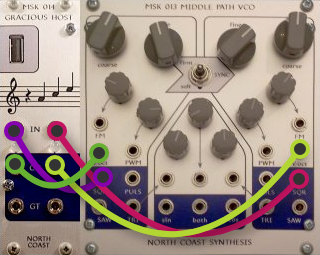
\includegraphics[scale=0.45]{calpatch1.png}\hspace*{\fill}\par} 

The module will automatically detect when a suitable VCO signal is present,
and will start sending different control voltages and measuring the
resulting frequencies.  It is trying to adjust the voltages for ten
different notes, while also re-confirming the frequency at 0V.  As more of
the voltages are detected as on-target, the red flashes get shorter while
keeping the same repetition rate of one flash every 1.05\,s.  When nearly
complete the LED will be off most of the time with only brief red flashes.

\blinkcodeX{}{0/2}

You can follow the progress of the output calibration by watching the length
of the flashes.  How long it takes depends on the VCO's stability and how
far the previous calibration was from the new one, but it is normally
expected to complete in less than a minute, and it may be only two or three
seconds if the previous calibration almost perfectly matches the new one.

When output calibration completes the channel will wait to be repatched for
input calibration.

\section{Input calibration}

When the channel is ready for input calibration it switches to a
faster blink pattern in alternating green and red.

\blinkcodeX{0/3.5}{4/7.5}

For this step, disconnect the VCO and just patch the Gracious Host's analog
output directly to its own analog input on the same side.  This diagram,
like the last one, shows both channels so patched, but remember that the
channels are independent and you can do input calibration on one of them
while the other is at a different stage.

\nopagebreak\noindent
{\hspace*{\fill}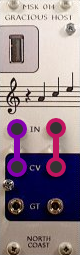
\includegraphics[scale=0.45]{calpatch2.png}\hspace*{\fill}\par} 

In principle, the input calibration will shorten its LED blinks to indicate
progress, in the same way that the output calibration did.  However, the
input calibration is usually so fast (two or three seconds per channel) that
you may not see the shorter blinks before it finishes.

\blinkcodeX{0/0.5}{4/4.5}

When one channel has completed input calibration, it will display quite fast
green blinks (3.8\,Hz, 50\% duty cycle) while it waits for the other.

\blinkcodeX{0/1,2/3,4/5,6/7}{}

When \emph{both} channels complete input calibration, both LEDs will go
solid green as part of the \emph{success display}, and the digital output
jacks will play a happy tune in 0V--9V square waves.  You can patch either
output jack to a speaker or headphone (remaining aware of the 4.5V DC
offset) to hear this.

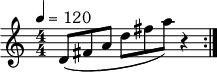
\includegraphics{success.cropped.eps}

\blinkcodeLR{0/8}{}{0/8}{}

The success display lasts one minute, after which the module will reboot. 

If you initiated calibration by doing a firmware update, then you ought to
have already disconnected the USB drive before the end of the success
display; otherwise, on reboot it will attempt to update the firmware again. 

The calibration data is written to the module's non-volatile memory at the
\emph{start} of the success display, so it is safe to power down the module
as soon as you see the solid green LEDs.  If you wish to abort calibration
once started, just power the module down before reaching the end.  In that
case, the module will end up with the default values from the firmware you
loaded, if you loaded firmware; or no change to the existing calibration if
you started calibration in some other way, such as with maintenance code
5833.
